\section{Balanceamento de árvores binárias}

\begin{frame}[fragile]{Balanceamento}

	\begin{itemize}
		\item Uma árvore binária está balanceada se a diferença de altura das duas subárvores de 
            qualquer nó da árvore é menor ou igual a 1

        \item Uma árvore binária está perfeitamente balanceada se ela está balanceada e todos os 
            seus nó se encontram em, no máximo, dois níveis distintos

        \item Uma árvore binária é dita completa se está perfeitamente balanceada 
            e as folhas do seu último nível estão mais à esquerda possível

        \item Uma árvore binária é dita cheia se todos os seus nós tem ou zero ou dois filhos

        \item A altura de uma árvore é igual ao nível máximo dentre todos os nós da árvore

        \item Uma árvore pode estar balanceada sem estar perfeitamente balanceada
	\end{itemize}

\end{frame} 
 

\begin{frame}[fragile]{Exemplo de árvore desbalanceada}

    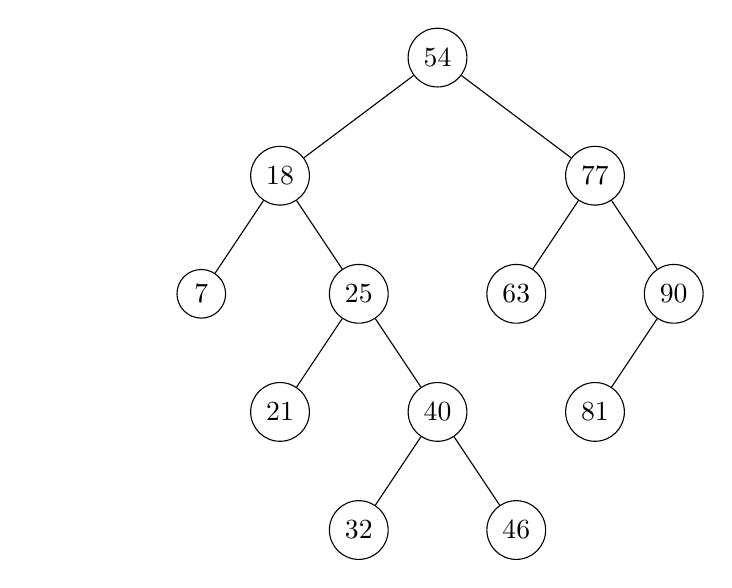
\begin{tikzpicture}
        \begin{scope}{shift={(3,0)}}
            \node[opacity=0] (X) at (-1, 2) { $1$ };
            \node[circle,draw] (A) at (4, 8) { 54 };
            \node[circle,draw] (B) at (2, 6.5) { 18 };
            \node[circle,draw] (C) at (6, 6.5) { 77 };
            \node[circle,draw] (D) at (1, 5) { 7 };
            \node[circle,draw] (E) at (3, 5) { 25 };
            \node[circle,draw] (F) at (5, 5) { 63 };
            \node[circle,draw] (G) at (7, 5) { 90 };
            \node[circle,draw] (H) at (2, 3.5) { 21 };
            \node[circle,draw] (I) at (4, 3.5) { 40 };
            \node[circle,draw] (J) at (6, 3.5) { 81 };
            \node[circle,draw] (K) at (3, 2) { 32 };
            \node[circle,draw] (L) at (5, 2) { 46 };

            \draw (A) -- (B);
            \draw (A) -- (C);
            \draw (B) -- (D);
            \draw (B) -- (E);
            \draw (C) -- (F);
            \draw (C) -- (G);
            \draw (E) -- (H);
            \draw (E) -- (I);
            \draw (G) -- (J);
            \draw (I) -- (K);
            \draw (I) -- (L);

        \end{scope}
    \end{tikzpicture}

\end{frame}

\begin{frame}
\frametitle{Exemplo de árvore perfeitamente balanceada}

    \begin{tikzpicture}
        \begin{scope}{shift={(3,0)}}
            \node[opacity=0] (X) at (-1, 2) { $1$ };
            \node[circle,draw] (A) at (4, 8) { 13 };
            \node[circle,draw] (B) at (2, 6.5) { 10 };
            \node[circle,draw] (C) at (6, 6.5) { 25 };
            \node[circle,draw] (D) at (1, 5) { 2 };
            \node[circle,draw] (E) at (3, 5) { 12 };
            \node[circle,draw] (F) at (5, 5) { 20 };
            \node[circle,draw] (G) at (7, 5) { 31 };
            \node[circle,draw] (H) at (6, 3.5) { 29 };
%            \node[circle,draw] (I) at (4, 3.5) { 40 };
%            \node[circle,draw] (J) at (6, 3.5) { 81 };
%            \node[circle,draw] (K) at (3, 2) { 32 };
%            \node[circle,draw] (L) at (5, 2) { 46 };

            \draw (A) -- (B);
            \draw (A) -- (C);
            \draw (B) -- (D);
            \draw (B) -- (E);
            \draw (C) -- (F);
            \draw (C) -- (G);
            \draw (G) -- (H);
%            \draw (E) -- (I);
%            \draw (G) -- (J);
%            \draw (I) -- (K);
%            \draw (I) -- (L);

        \end{scope}
    \end{tikzpicture}

\end{frame}

\begin{frame}
\frametitle{Exemplo de árvore balanceada, mas não perfeitamente balanceada}

    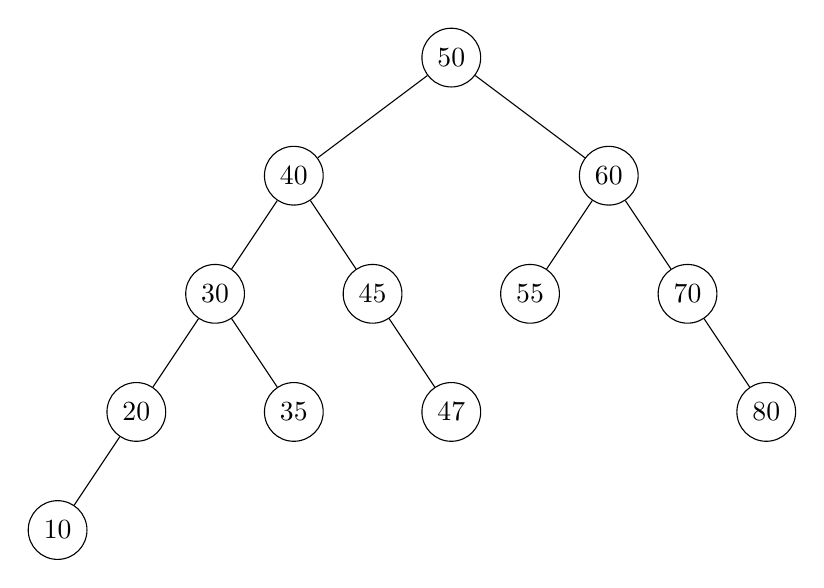
\begin{tikzpicture}
        \begin{scope}{shift={(3,0)}}
            \node[opacity=0] (X) at (-1, 2) { $1$ };
            \node[circle,draw] (A) at (4, 8) { 50 };
            \node[circle,draw] (B) at (2, 6.5) { 40 };
            \node[circle,draw] (C) at (6, 6.5) { 60 };
            \node[circle,draw] (D) at (1, 5) { 30 };
            \node[circle,draw] (E) at (3, 5) { 45 };
            \node[circle,draw] (F) at (5, 5) { 55 };
            \node[circle,draw] (G) at (7, 5) { 70 };
            \node[circle,draw] (H) at (0, 3.5) { 20 };
            \node[circle,draw] (I) at (2, 3.5) { 35 };
            \node[circle,draw] (J) at (4, 3.5) { 47 };
            \node[circle,draw] (K) at (8, 3.5) { 80 };
            \node[circle,draw] (L) at (-1, 2) { 10 };

            \draw (A) -- (B);
            \draw (A) -- (C);
            \draw (B) -- (D);
            \draw (B) -- (E);
            \draw (C) -- (F);
            \draw (C) -- (G);
            \draw (D) -- (H);
            \draw (D) -- (I);
            \draw (E) -- (J);
            \draw (G) -- (K);
            \draw (H) -- (L);

        \end{scope}
    \end{tikzpicture}

 \end{frame}
 
\begin{frame}[fragile]{Algoritmo para verificação de balanceamento}

	\begin{itemize}
        \item É possível utilizar a recursão para checar o balanceamento a cada nó,
            usando também a rotina recursiva de cálculo de tamanho

        \item O algoritmo é de fácil entendimento, mas possui maior complexidade
            assintótica $O(N^2)$
	
        \item É possível reduzir a complexidade para $O(N)$ através do uso de programação dinâmica

        \item Para verificar se uma árvore está perfeitamente balanceada, primeiro é 
                necessário verificar se a mesma está balanceada

        \item Em seguida, determina-se a altura da árvore: se ela não extrapolar o menor inteiro 
            maior do que $\log(N + 1)$, a árvore está perfeitamente balanceada
	\end{itemize}

\end{frame}

\begin{frame}[fragile]{Implementação do algoritmo de verificação de balanceamento}
    \inputsnippet{cpp}{1}{17}{is_balanced.cpp}
\end{frame}

\begin{frame}[fragile]{Implementação do algoritmo de verificação de balanceamento}
    \inputsnippet{cpp}{18}{38}{is_balanced.cpp}
\end{frame}
